\section{Introduction} \label{sec:dev_intro}

%%%%%%%%%%%%%%%%%%%%%%%%%%%%%%%%%%%%%%%
\subsection{Motivations}
%%%%%%%%%%%%%%%%%%%%%%%%%%%%%%%%%%%%%%%
    
    Le domaine du HPC est en pleine croissance et les utilisateurs ont besoin d'architectures toujours plus puissantes pour analyser le tsunami de données produit par les objets connectés, prendre des décisions plus complexes (voiture autonome) et plus rapides (éviter un accident). Cependant, plusieurs contraintes ralentissent l'évolution des architectures dont les principales concernent l'énergie (loi de Moore, évolution de Dennard). Les 10 premiers supercalculateurs du Top500[1] consomment entre 7 et 20 MW quand l'objectif est de construire un supercalculateur Exascale (10 fois plus puissant) consommant entre 20 et 30 MW. Il n'est donc plus viable de garder la même tactique qui consiste à doubler le nombre de serveurs pour obtenir des clusters deux fois plus puissant.
    
    Les différentes nouvelles technologies présentées dans la \autoref{sec:edl_opportunite} vont permettre le développement d'une multitude de nouvelles architectures très différentes et encore plus complexes que celles utilisées aujourd'hui. Grâce au protocole Gen-Z, de nombreuses technologies pourront être utilisées pour exécuter les différents noyaux d'une application de façon optimale. La principale piste pour la construction d'une plateforme Exascale est d'utiliser ces architectures ultra-optimisées pour certains noyaux de calculs exécutés.
    
    L'amélioration de la performance énergétique ne viendra pas seulement des architectures, mais aussi de la capacité des codes à les utiliser correctement, ce qui est loin d'être le cas aujourd'hui. La plupart des supercalculateurs atteignent rarement 80\% d'efficacité sur une application simple comme Linpack\cite{Dongarra2003}. Pour des applications réelles, cette efficacité est encore plus faible, parfois inférieure à 10\%\cite{Oliker2005}. La principale source de consommation d'énergie ne provient pas du calcul, mais du déplacement des données\cite{Kothe2016}, l'optimisation de ces transferts est donc cruciale. De plus, comme la performance de la plupart des applications scientifiques est limitée par la bande passante mémoire, le travail de compréhension et d'optimisation est naturellement devenu la préoccupation de nombreux chercheurs et ingénieurs\cite{McCalpin1995}.
    


    \subsubsection{Objectifs}
    %%%%%%%%%%%%%%%%%%%%%%%%%%%%%%%%%%%%%%%

        L'hétérogénéité des centres de calculs est l'unique solution pour l'élaboration de plateformes Exascale. Cependant cela nécessite d'avoir recours à de nouvelles architectures très différentes de celles utilisées aujourd'hui (x86, GPU). Ces architectures doivent ainsi être caractérisées pour pouvoir y porter les applications et vérifier que les performances optimales sont atteintes. Une fois les plateformes et les noyaux de calculs caractérisés, le programmeur peut estimer le coût de portage d'une application. Cette mesure est à la fois un coût économique (prix de la plateforme, consommation électrique), mais aussi de temps pour réaliser la transformation de code nécessaire.
        
        Pour réaliser ce travail de caractérisation et d'optimisation, le programmeur doit avoir à sa disposition différents outils. Une première famille composée de code de benchmark lui permet de caractériser une nouvelle architecture pour en connaître les principales caractéristiques et estimer son efficacité pour une application. 
        Il doit ensuite utiliser un deuxième jeu d'outils pour obtenir le profil de son application. Chaque application HPC possède plusieurs zones de calculs intensifs qui peuvent avoir des caractéristiques différentes. Pour choisir la plateforme optimale pour l'un d'entre eux, le programmeur doit posséder un outil lui permettant d'extraire et de caractériser ces zones de codes.
        
      

%%%%%%%%%%%%%%%%%%%%%%%%%%%%%%%%%%%%%%%%%%%%%%%%%
\subsection{Contributions}
%%%%%%%%%%%%%%%%%%%%%%%%%%%%%%%%%%%%%%%%%%%%%%%%%

        Pour pouvoir en bénéficier de l'hétérogénéité et de la multitude de nouvelles architectures disponibles, nous proposons une méthodologie en 5 étapes. Celle-ci permet d'identifier et caractériser ces nouvelles plateformes, de modéliser la performance d'une application, pour enfin porter son code sur l'architecture choisie et en extraire la performance maximale. La méthodologie est résumée sur la \autoref{pic:methodologie_step_1} et présentée dans le \autoref{chap:methodo}.

        \begin{figure}[h!]
        \center
        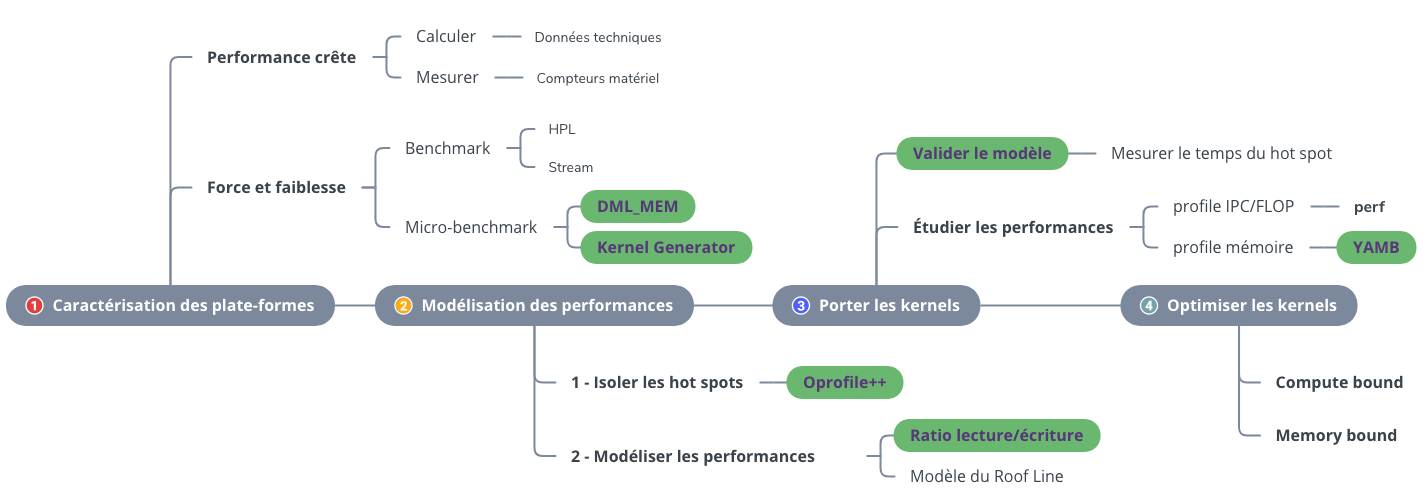
\includegraphics[width=16cm]{images/methodologie_step.png}
        \caption{\label{pic:methodologie_step_1} Méthodologie en 5 étapes pour caractériser et optimiser une application sur une nouvelle architecture.}
        \end{figure}
        
        Pour chaque étape, nous avons sélectionné les outils nécessaires pour répondre aux questions permettant de poursuivre la méthodologie. Pour cela nous avons réalisé un état de l'art des outils existant, sélectionné ceux répondant à nos critères de développement et développé ceux manquants.
        
        
   
    \subsubsection{Travaux existants}
    %%%%%%%%%%%%%%%%%%%%%%%%%%%%%%%%%%%%%%%%%%%%%%%%%%%%%%%%%%%%%%%%%%%%%%%%
    
        \paragraph{Les outils de suivi de performance.} Les évènements se produisant sur un processeur peuvent être comptés à l'aide de compteurs matériels. Ils sont accessibles par le biais de composants appelés Performance Monitor Units (PMU). Sur les CPU modernes, il y a au moins deux PMU : une sur le noyau et une sur le socket responsable des évènements qui s'y rapportent (comme l'accès mémoire). Ces compteurs varient d'une architecture à l'autre, ou d'un modèle de processeur à l'autre, ce qui les rend difficiles à programmer et à maintenir. Que ce soit pour le core ou le uncore, ces méthodes sont assez complexes à utiliser et à maintenir. C'est pourquoi nous utilisons des interfaces de haut niveau telles que \textit{PAPI} ou \textit{perf} qui nous permettent de ne plus dépendre de l'implémentation des compteurs à bas niveau. 
        
        De nombreux outils ont été développés pour suivre l'activité du CPU (voir \autoref{sec:edl_monitoring_tools}). Certains sont propriétaires comme \verb|VTune|\cite{reinders2005vtune} et nécessitent des licences payantes. D'autres nécessitent des droits supplémentaires (\textit{root} ou noyau) pour être utilisés. D'autres outils sont proposés en sources libres, mais ne sont compatibles qu'avec un nombre limité d’architectures \verb=x86=. Enfin, des outils tels que \verb=TAU= ou \verb=Extrae= présentent de nombreuses informations à l'utilisateur qui rendent difficile la compréhension des résultats. De plus, ce grand nombre d'informations nécessite généralement l'utilisation de plusieurs compteurs matériels qui peuvent ne plus être présents d'une architecture ) l'autre. La complexité des outils peut aussi les rendre dépendants de librairies externes non compatibles avec certaines architectures rendant leur utilisation impossible (\verb|MAQAO|).

        \paragraph{Les benchmarks.} Pour découvrir les caractéristiques d'une architecture, il est courant d'utiliser des programmes artificiels, appelés benchmarks, pour effectuer un certain type d'opération ou reproduire la même charge de travail qu'une application réelle. En HPC, deux benchmarks sont largement utilisés : le High Performance Linpack (HPL) \cite{Dongarra2003} mesure le taux d'exécution en virgule flottante pour résoudre un système d'équations linéaire. Le second, STREAM \cite{McCalpin1995}, est utilisé pour mesurer la bande passante mémoire durable pour un simple benchmark synthétique. Pour mieux représenter les applications réelles et avoir un classement des supercalculateurs, des suites de plusieurs benchmarks sont également utilisées telles que HPC Challenge \cite{Ang2016} ou HPCG \cite{dongarra2016high}. Pour caractériser plus précisément une partie de la microarchitecture, on peut utiliser d'autres codes tels que \textit{lmbench}. \cite{Staelin2004}. Il est composé de deux familles de benchmarks : une pour la bande passante mémoire et une pour la latence. Par exemple, il est capable de mesurer la latence de chaque niveau de cache de la mémoire. En raison de son incapacité à mesurer les performances du cache distant et les transactions de cohérence du cache, le benchmark \textit{x86-membench} benchmark \cite{Molka2017b} a été développé pour supporter la mesure de la bande passante et de la latence du cache local ou distant, mais aussi de la mémoire. 
        
    \subsubsection{Critères de développement}
    %%%%%%%%%%%%%%%%%%%%%%%%%%%%%%%%%%%%%%%%%%%%%%%%%%%%%%%%%%%%%%%%%%%%%%%%
        
        Pour sélectionner et développer les outils nécessaires à ce travail, une liste de critères a été établie. Ces critères permettent d'assurer le maximum de productivité en répondant à des questions simples. Bien que certains travaux déplorent l'absence d'outils automatiques \cite{Chung2012}, nous estimons que la complexité des architectures et les multiples facteurs impactant la performance rendent impossible le développement d'un tel outil. Au contraire, notre philosophie de développement repose sur l'utilisation d'outils simples répondant à une question précise. En développant des outils simples, le programmeur peut facilement en comprendre le déroulement et se l'approprier en apportant les modifications qu'il estime judicieuses. En proposant les outils en source ouverte, nous espérons que l'expérience des différents utilisateurs puisse profiter au reste de la communauté.
        
        L'objectif de notre travail est la caractérisation de nouvelles plateformes, différentes de celles utilisées actuellement. Un critère majeur pour nos développements est d'assurer la compatibilité avec le maximum d'architectures. Le développement d'outils simples facilite d'autant plus la tâche du portage des outils. Ce critère interdit donc l'utilisation d'outils tels de \verb=VTune=, utilisable uniquement pour les architectures Intel.
        
        Le travail de caractérisation est une tâche très complexe, si l'utilisation des outils doit être facilitée, il ne faut pas négliger la facilité d'installation. Plusieurs retours d'expérience nous ont montré que de nombreux utilisateurs n'utilisent pas certains outils lorsqu'ils ne parviennent pas à l'installer au premier essai. La réduction des dépendances à des librairies externes, et le développement d'outils simple nous assure de réduire les difficultés lors de l'installation. De plus, dans des environnements industriels, l'utilisateur n'a pas toujours la liberté d'installer toutes les librairies qu'il souhaite pouvant ainsi l'empêcher d'installer un outil. 
        Les programmeurs qui travaillent quotidiennement sur des supercalculateurs savent que l'installation d'un outil, même simple, peut prendre du temps et de l'énergie : qu'il s'agisse de scripts de compilation complexes à déboguer ou de la dépendance à d’anciennes versions de bibliothèque. Pour ce faire, nos outils développés sont basés sur le nombre minimum de bibliothèques et l'outil de gestion de compilation libre de droits \textit{cmake}. CMake fait automatiquement la découverte et la configuration de la chaîne d'outils ce qui augmente la \textbf{portabilité} du code. 

        Dans un environnement industriel, l'utilisateur n'aura pas non plus accès à des droits supplémentaires (\textit{root} ou \textit{kernel}). Nous avons donc sélectionné et développé des outils ne nécessitant pas ces droits. Les compteurs matériels nécessitent des droits privilégiés, empêchant l'utilisation de nombreux outils existants. Cette raison est la principale motivation de l'utilisation du \textit{backend} de \verb=Perf Events= qui peut être rendu accessible à n'importe quel utilisateur. Bien que cette commande doive être exécutée par l'utilisateur \verb=root=, elle ne doit être exécutée qu'une seule fois à l'allumage de la machine:\\
        \verb|sudo sh -c 'echo 1 >/proc/sys/kernel/perf_event_paranoid'|\\
        
        Comme présenté dans la \autoref{sec:edl_hc_conclusion}, les compteurs matériels souffrent d'un manque de compatibilité entre les architectures (même d'un même constructeur) et peuvent être indisponibles sur des architectures de nouvelle génération. Les difficultés de programmation exprimées dans l'état de l'art nous ont contraints à ne sélectionner que des outils ne se basant que sur des compteurs matériels standards. De plus, l'utilisation de compteurs plus complexes ne permet pas toujours de conclure facilement de la bonne ou mauvaise performance d'un code. Par exemple, un grand nombre de \textit{miss} dans le cache de niveau 1 n'implique pas forcément une mauvaise performance s'il s'agit d'un algorithme de \textit{stream}. Pour ces deux raisons nous avons choisi de n'utiliser et de développer des outils ne se basant que des évènements simples: nombre de cycles, nombre d'instructions exécutées, instructions mémoire en cours et nombre de \textit{miss} dans le dernier niveau de cache.
        
\subsection{Organisation du chapitre}
%%%%%%%%%%%%%%%%%%%%%%%%%%%%%%%%%%%%%%%%%%%%%%%%%%%%%%%%%%%%%%%%%%%%%%%%
   
    Ce chapitre présente les 4 principaux outils développés lors du travail de thèse. Il suit la structure suivante:
   
   \begin{itemize}
       \item La \autoref{sec:dmlmem} présente un nouveau benchmark permettant de réaliser des accès par sauts (strides) en mémoire pour des jeux de données de taille variable. Ce genre d'accès est très répandu dans les applications de type RTM et il est important de pouvoir caractériser la microarchitecture pour ces codes-là.
       \item La \autoref{sec:kg} introduit un générateur de benchmarks permettant de caractériser finement les unités de calcul arithmétique (ALU). Les architectures peuvent avoir des performances inégales et la performance de chaque instruction vectorielle doit être vérifiée pour valider la performance d'une application réelle (nombre d'instruction par cycle, fréquence supportée, opération flottante par seconde).
       \item La \autoref{sec:yamb} introduit un outil permettant de suivre l'évolution du trafic du bus mémoire. La mémoire étant une ressource critique des architectures modernes, cet outil est essentiel pour poursuivre la caractérisation des applications.
       \item La \autoref{sec:oprofile} présente un outil capable d'extraire le code assembleur des \textit{hot spots} d'une application et de caractériser chaque instruction ainsi que d'établir le résumé de la performance des boucles critiques.
   \end{itemize}
   
     
